\documentclass[titlepage]{article}

% Language setting
% Replace `english' with e.g. `spanish' to change the document language
\usepackage[english]{babel}

\usepackage{fancyhdr}

% Set page size and margins
% Replace `letterpaper' with`a4paper' for UK/EU standard size
\usepackage[letterpaper,top=2cm,bottom=2cm,left=3cm,right=3cm,marginparwidth=1.75cm]{geometry}

% Useful packages
\usepackage{amsmath}
\usepackage{graphicx}
\usepackage{physics}
\usepackage[colorlinks=true, allcolors=blue]{hyperref}

\usepackage[parfill]{parskip}

% tables
\usepackage{geometry}
\usepackage{makecell}
\usepackage{multicol}
\usepackage{float}
\usepackage{lscape}
\usepackage{amsmath}
\usepackage[font=small,labelfont=bf,justification=centering]{caption}

\setcellgapes{10pt}

\captionsetup[table]{justification=raggedright,singlelinecheck=off}

% \setlength{\parindent}{0pt}

\setcounter{tocdepth}{4}
\setcounter{secnumdepth}{4}

\usepackage{gensymb}

\usepackage{tgpagella}
\renewcommand{\familydefault}{\sfdefault}

\graphicspath{{images/}}

\title{AP Physics C: Mechanics - Notes}
\author{Manav Bokinala}
\date{2021 - 2022}

\pagestyle{fancy}
\fancyhf{}
\fancyhead[LE,RO]{Manav Bokinala}
\fancyhead[RE,LO]{AP Physics C: Mechanics - Notes}
\fancyfoot[LE,RO]{\thepage}

\begin{document}
\maketitle

\newpage
\tableofcontents
\newpage

\section{Vectors and Motion in 2 Dimensions}
Unit vector: length of 1, no units (used for direction)

\begin{itemize}
    \item Denoted with "hat"
    \item $\hat{x}$, $\hat{y}$, $\hat{z}$ - usually denoted as $\hat{i}$, $\hat{j}$, $\hat{k}$
\end{itemize}

For a 2D velocity vector:
\[ \vec{v} = v_x \hat{i} + v_y \hat{j} \]

\subsection{Polar Notation}
\[ \vec{v} = \sqrt{{v_x}^2 + {v_y}^2} \text{ at } \theta \degree \]

$\theta$ is angle relative to \emph{positive x-axis}

\subsection{Vector Addition}
\begin{align*}
    \vec{A}           & = A_x \hat{i} + A_y \hat{j}                 \\
    \vec{B}           & = B_x \hat{i} + B_y \hat{j}                 \\
    \vec{A} + \vec{B} & = (A_x + B_x) \hat{i} + (A_y + B_y) \hat{j}
\end{align*}

\subsection{Scalar Multiplication}
scalar $\cdot$ vector = vector

\begin{align*}
     & \vec{A} = A_x \hat{i} + A_y \hat{j}    \\
     & 2\vec{A} = 2A_x \hat{i} + 2A_y \hat{j}
\end{align*}

\subsection{Vector Multiplication}
vector $\cross$ vector\\

scalar/dot product: $\vec{A} \cdot \vec{B}$
\begin{itemize}
    \item results in scalar
\end{itemize}

vector/cross product: $\vec{A} \cross \vec{B}$
\begin{itemize}
    \item results in vector
\end{itemize}

\subsection{Dot Product}
\[
    \vec{A} \cdot \vec{B} = \abs{A} \abs{B} \cos \theta
\]

\begin{itemize}
    \item $\theta$ is the angle between the two vectors
\end{itemize}

Or,

\[ \vec{A} \cdot \vec{B} = A_xB_x + A_yBy \]

\subsubsection{Dot Product Properties}
\begin{align*}
    \vec{A} \cdot \vec{B} & = \vec{B} \cdot \vec{A}                               \\
    \vec{A} \cdot \vec{B} & = 0 \text{ if $\vec{A}$ and $\vec{B}$ are orthogonal}
\end{align*}

\subsection{Cross Products}
\begin{align*}
    \text{If } \vec{C} & = \vec{A} \cross \vec{B},     \\
    \abs{C}            & = \abs{A} \abs{B} \sin \theta
\end{align*}

the cross product is \textbf{orthogonal} to both original vectors (uses 3rd dimension)

\subsubsection{Cross Product Properties}

\begin{align*}
     & \vec{A} \cross \vec{B} \neq \vec{B} \cross \vec{A} \\
     & \vec{A} \cross \vec{B} = - \vec{B} \cross \vec{A}
\end{align*}

right hand rule - cross product goes "into" or "out of" page

\section{Drag Force}
\begin{itemize}
    \item resistive force by \textbf{\emph{fluids}} on \textbf{\emph{moving objects}}
    \item \textbf{\emph{opposes}} direction of motion
\end{itemize}

\subsection{\texorpdfstring{$v^2$}{v\^{}2} model}
\[ F_{drag} = - \frac{1}{2} C \rho A v^2 \]

\begin{itemize}
    \item $C$ - drag coefficient
    \item $\rho$ - density of fluid - greek letter "rho"
    \item $A$ - cross-sectional area of object
    \item $v$ - velocity of object
    \item negative sign just indicates direction opposite to motion
\end{itemize}
\ \\
Sometimes, the coefficients $\frac{1}{2}C \rho A v^2$ are grouped into one coefficient ($b$ or $k$)

\begin{itemize}
    \item So, $F_{drag} = -bv^2$
    \item also called the drag coefficient
    \item specific to object and location
    \item calculated experimentally
\end{itemize}

\subsection{\texorpdfstring{$v$}{v} model}
for \textbf{\emph{small objects}} moving at \textbf{\emph{slow speeds}},
\[F_{drag} = -bv\]

\subsection{Terminal Velocity}
For an object in free fall, terminal velocity occurs when $\abs{\vec{F}_{drag}} = \abs{\vec{F}_{gravity}}$

\begin{align*}
    F_{net} & = F_g - F_{drag}                             \\
    0       & = mg - bv_t                                  \\
    v_t     & = \frac{mg}{b} \text{ ($v$ model)}           \\
    v_t     & = \sqrt {\frac{mg}{b}} \text{ ($v^2$ model)}
\end{align*}

\section{Differential Equations}
Differential equations define relationship between a function and one or more \emph{derivatives} of that function

Drag force is modeled with a differential equation:

\begin{align*}
    F_{drag}        & = bv \\
    ma              & = bv \\
    % \frac{d}{dt} \left[ ma \right] &= \left[ bv \right] \\
    m \frac{dv}{dt} & = bv
\end{align*}

\subsection{Integrating Differential Equations}
\begin{align*}
    m \frac{dv}{dt}     & = bv               &  & \text{rewrite equation to see dependent and independent variables} \\
    \frac{1}{v} dv      & = \frac{b}{m} dt   &  & \text{separate each variable to one side}                          \\
    \int \frac{1}{v} dv & = \int \frac{b}{m} &  & \text{integrate}
\end{align*}

\section{Circular Motion}
Centripetal force ($F_c$ or $\sum F_c$) isn't really a force - it is the \textbf{net} force along the centripetal axis (the axis going through a point on the circular path and the center of said circle).
\begin{itemize}
    \item could be weight, tension, friction, etc.
    \item is always orthogonal (perpendicular) to velocity
    \item depends on mass and tangential velocity of object and radius of circular path
\end{itemize}

\subsection{Uniform Circular Motion}
Uniform circular motion occurs when an object moving in a circle with a fixed radius has a constant tangential (and therefore angular) speed

\textbf{frequency} ($f$) is measured in Hertz {Hz}\\
\textbf{period} ($T$) is measured in seconds (s)

\subsection{Velocity}
\[v_t = \frac{\Delta x}{T} = \frac{2\pi r}{T} = 2\pi rf\]

\subsection{Acceleration}
\[a_c = \frac{v^2}{r} = \frac{4 \pi^2 r}{T^2}\]

Centripetal acceleration always points toward the center of the circular path
\begin{itemize}
    \item does not change \emph{speed} of object; only changes \emph{direction}
\end{itemize}

\subsection{Force}
Centripetal force is the sum of all forces on the centripetal axis

\begin{align*}
    \sum F   & = ma             \\
    \sum F_c & = ma_c           \\
    \sum F_c & = \frac{mv^2}{r}
\end{align*}

points toward the center of the circular path

\section{Rotational Motion}

\textbf{rigid bodies}: objects that do not change shape (deform)\\
\textbf{translational motion}: motion of the \emph{center of mass} of the object\\
\textbf{rotational motion}: rotation around a fixed point (not always the center of mass)
\ \\
\begin{table}[H]
    \makegapedcells
    \begin{tabular}{c|c}
        \textbf{Circular Motion}                    & \textbf{Rotational Motion}                                \\
        \hline

        circular path                               & spins about axis of rotation                              \\
        all parts of object move with same velocity & different points on the object travel at different speeds \\
    \end{tabular}
\end{table}

\subsection{Variables}
\begin{itemize}
    \item $R$ - distance from point on object to axis of rotation
    \item $\theta$ - angular displacement - \emph{measured in radians}
    \item $S$ - Arc Length
\end{itemize}
\[S = R\theta\]

\subsection{Angular Velocity}
rate of change of $\theta$
\[ \omega = \frac{\Delta \theta}{t} = 2 \pi f \]

\begin{itemize}
    \item $\omega$ - angular velocity - \emph{measured in radians/second}
\end{itemize}
\ \\
all points on a rigid body have the same angular velocity

$\omega$ does \textbf{\emph{not}} point in the direction of rotation
\begin{itemize}
    \item use the right hand rule to determine the direction of $omega$ - always orthogonal to the rotational plane
          \begin{itemize}
              \item usually described as "into page" or "out of page"
              \item sometimes described as "clockwise" or "counterclockwise"
          \end{itemize}
\end{itemize}

\subsection{Angular Acceleration}
rate of change of $omega$
\[ \alpha = \frac{\Delta \omega}{t} \]
\begin{itemize}
    \item $\alpha$ - angular acceleration - \emph{measured in radians/second\textsuperscript{2}}
\end{itemize}
\ \\
$\alpha$ does \textbf{\emph{not}} point in the direction of rotation - same as angular velocity ($\omega$)
\begin{itemize}
    \item use right hand rule just like angular velocity to determine direction of $\alpha$
\end{itemize}

\subsection{Kinematic Equations}

\begin{table}[H]
    \makegapedcells
    \begin{tabular}{c|c}
        \textbf{Translational Kinematics}    & \textbf{Rotational Kinematics}                         \\
        \hline
        $\bar{v} = \dfrac{\Delta x}{t}$      & $\bar{\omega} = \dfrac{\Delta \theta}{t}$              \\
        $\bar{v} = \dfrac{v_1 + v_2}{2}$     & $\bar{\omega} = \dfrac{\omega_1 + \omega_2}{2}$        \\
        $\bar{a} = \dfrac{v - v_0}{t}$       & $\bar{\alpha} = \dfrac{\omega - \omega_0}{t}$          \\
        $\Delta x = v_0 t + \frac{1}{2}at^2$ & $\Delta \theta = \omega_0 t + \frac{1}{2} \alpha t^2$  \\
        ${v_{f}}^2 = {v_0}^2 + 2a\Delta x$   & ${\omega_{f}}^2 = {\omega_0}^2 + 2\alpha\Delta \theta$ \\
    \end{tabular}
\end{table}

\section{Center of Mass (Discrete Objects)}
\begin{itemize}
    \item The point at which all \textbf{mass} of an object is though to be concentrated
    \item also thought of as "average location of mass"
    \item can be determined experimentally or mathematically
    \item the center of mass of \emph{all objects} moves like a point particle \emph{even if the object is rotating}
    \item could be inside or outside the object
    \item the geometric center of an object is \emph{not} always its center of mass - only when the object has a uniform density
    \item unless specified, objects have a uniform density
\end{itemize}

\subsection{Position of the Center of Mass}
\[x_{cm} = \frac{1}{M}\sum m_i x_i\]

\begin{itemize}
    \item $x_cm$ = position of the center of mass of the systeme
    \item $M$ - total mass of the systeme
    \item $m_i$ - mass of the $i$\textsuperscript{th} particle
    \item $v_i$ - psoition of the $i$\textsuperscript{th} particle
\end{itemize}

A continuous object can be broken down into symmetric discrete pieces to find its center of mass

\subsection{Velocity of the Center of Mass}
\[v_cm = \frac{1}{M}\sum m_i v_i\]

\begin{itemize}
    \item $v_i$ - velocity of the $i$\textsuperscript{th} particle
\end{itemize}

\subsection{Acceleration of the Center of Mass}
Newton's third law ($F = ma$) actually refers to the center of mass of a system or object:
\[Ma_{cm} = \sum F_{external}\]

\section{Center of Mass (Continuous Objects)}
Not all continuous objects have a uniform mass density
\begin{itemize}
    \item Mass density usually varies with location
\end{itemize}

\[x_{cm} = \frac{1}{M} \int x \ dm\]
\begin{itemize}
    \item $x$ - position of particle
    \item $dm$ - infinitely small mass
\end{itemize}
position is given as a function of mass\\
integrate along the length of the object

\subsection{Position of Center of Mass}
\begin{enumerate}
    \item Define mass density function: \[\lambda = \frac{dm}{dx}\]
    \item Separate variables: \[dm = \lambda(x) dx\]
    \item Integrate along length of object to find total mass of object:
    \item Use integral form of center of mass formula (see above) to solve for the position of the center of mass
          \begin{itemize}
              \item use total mass calculated in step 4
          \end{itemize}
\end{enumerate}

\section{Rotational Intertia}
Rotational inertia (a.k.a \textbf{moment of inertia}): ability of an object to resist changes in its rotational motion\\ \\
symbol: $I$\\
scalar quantity\\
units: kg $\cdot$ m$^2$

\subsection{Discrete Objects}
\begin{equation*}
    I = \sum m_i R_i^2
\end{equation*}

\begin{itemize}
    \item $m_i$ - mass of object
    \item $R$ - distance between axis of rotation and the object
\end{itemize}

The same object can have different rotational inertias depending on the location of the axis of rotation

\subsection{Continuous Objects}
\begin{equation*}
    I = \int R^2 \ dm
\end{equation*}

\begin{table}[H]
    \centering
    \makegapedcells

    \begin{tabular}{c|c}
        \textbf{Object and Axis of Rotation} & \textbf{Rotational Inertia} \\
        \hline
        Thin rod, about center               & $\frac{1}{12}ML^2$          \\
        Thin rod, about end                  & $\frac{1}{3}ML^2$           \\
        Cylinder or disk, about center       & $\frac{1}{2} MR^2$          \\
        Cylindrical hoop, about edge         & $MR^2$
    \end{tabular}
\end{table}

\subsection{Parallel Axis Theorem}
If the moment of inertia about the center of mass ($I_{CoM}$) is known, the moment of inertia about any parallel axis of rotation can be found using the formula:
\begin{equation*}
    I_{parallel} = I_{CoM} + Md^2
\end{equation*}

\begin{itemize}
    \item $M$ - mass of the objects
    \item $d$ distance between the axes
\end{itemize}

\subsection{Systems of Objects}
For a system of discrete and/or continous objects:
\begin{equation*}
    I_{system} = I_1 + I_2 + I_3 + \cdots + I_n
\end{equation*}

\section{Torque}
\textbf{Torque} is the ability of a force to make an object rotate - a "twisting force"

symbol: $\tau$ ("tau") \\
units: $N \cdot m$ \\
vector quantity

Magnitude depends on
\begin{itemize}
    \item size of the force
    \item direction
    \item location at which the force is applied
\end{itemize}

torque is given as the cross product $R \cross F$:
\begin{equation*}
    \tau = R \cross F = RF \sin \theta
\end{equation*}

\begin{itemize}
    \item $R$ - distance from the axis of rotation to the applied force
    \item $F$ - applied force
    \item $\theta$ - angle between $R$ and $F$ (when drawn tip-to-tail)
\end{itemize}

\subsection{Direction of Torque}
Use the right hand rule to find the direction of torque:
\begin{itemize}
    \item point index finger in direction from axis of rotation to applied force
    \item point middle finger in direction of applied forces
    \item point thumb out - this is the direction of the torque
\end{itemize}

\subsection{Torque in Newton's Second Law}
\begin{align*}
    \tau_{net} & = R \cross F                                            \\
               & = R F_{net}                                             \\
               & = Rma         &  & \text{Newton's 2nd Law, } F = ma     \\
               & = Rm \alpha R &  & a = \alpha R                         \\
               & = I \alpha    &  & \text{rotational inertia, } I = mR^2
\end{align*}

\section{Rolling}
Friction causes a torque that makes objects roll. Rolling objects experience both \textbf{rotational} and \textbf{translational} motion.

Objects can roll with or without \textbf{slipping}

\subsection{Rolling Without Slipping}
When an object rolls without slipping,
\begin{align*}
    v_{cm} = \omega R \\
    a_cm = \alpha R
\end{align*}

\begin{itemize}
    \item $v_{cm}$ and $a_{cm}$ are the velocities and accelerations of the center of mass, respectively
    \item $\omega$ and $\alpha$ are the angular velocity and acceleration of the object, respectively
    \item $R$ is the distance from the axis of rotation to the point of contact with the ground
\end{itemize}

Rolling without slipping problems are solved by relating the rotational and translational motions of an object using the equation $a = R\alpha$

\subsection{Rolling With Slipping}
When an object rolls without slipping,
\begin{align*}
    v_{cm} \neq \omega R \\
    a_{cm} \neq \alpha R
\end{align*}

Rolling without slipping problems are solved by figuring out \textbf{when} $v = R \omega$ (the object enters into rolling without slipping)

\subsubsection{Two Types of Rolling With Slipping}
\begin{enumerate}
    \item $v_{cm} > \omega R$ - object is sliding around ground at some points (e.g. bowling ball sliding and rolling slightly before it 'catches grip' and rolls at full speed)
    \item $v_{cm} < \omega R$ - object is spinning more than one revolution in the time it takes to advance by one circumference (e.g. car doing burnouts or losing traction)
\end{enumerate}

\section{Work and Energy}
\begin{itemize}
    \item energy is a scalar quantity (has no direction), but can be positive or negative'
    \item energy is always conserved in a closed system
\end{itemize}

\subsection{Work}
Work is the result of a force being applied to move an object across a displacement - measured in $N \cdot m$
\begin{equation*}
    W = F \cdot \Delta x = F \Delta x \cos \theta
\end{equation*}
\begin{itemize}
    \item work is the \textbf{cross product} of force and displacement (vector quantity)
    \item $\theta$ is the angle between $F$ and $\Delta x$ when aligned tail to tail
\end{itemize}

\subsubsection{Work-Energy Theorem}
Work changes the energy of an object
\begin{equation*}
    \Sigma W = \Delta KE
\end{equation*}
\begin{itemize}
    \item net work is equal to the change in kinetic energy of an object
\end{itemize}

\subsection{Energy}
Energy is measured in Joules ($J$) - equal to ($N \cdot m$)
\subsubsection{Types of Mechanical Energy}

\textbf{Kinetic Energy}
\begin{equation*}
    KE = \frac{1}{2}mv^2
\end{equation*}

\textbf{Rotational Kinetic Energy}
\begin{equation*}
    RKE = \frac{1}{2} I \omega ^ 2
\end{equation*}

\textbf{Potential Energy} \\
\emph{Gravitational}
\begin{equation*}
    GPE = mgh
\end{equation*}

\emph{Elastic}
\begin{equation*}
    EPE = \frac{1}{2}k (\Delta s)^2
\end{equation*}
\begin{itemize}
    \item $k$ - spring constant
    \item $\Delta s$ - displacement of the spring (compression or extension)
\end{itemize}

\subsection{Power}
power is energy delivered over a period of time

\begin{equation*}
    P = \frac{\Delta E}{\Delta t} = \frac{W}{\Delta t} = \frac{F \Delta x}{\Delta t} = Fv
\end{equation*}

\subsection{Potential Energy Curves}
graph of potential energy vs position

For \textbf{conservative forces},
\begin{equation*}
    F(x) = -\frac{d}{dx} U(x)
\end{equation*}

\subsubsection{Equilibrium Points}
Occur where the slope (equal to $F_{net}$) is zero


\section{Impulse and Momentum}
\textbf{impulse} is a force applied for a period of time

symbol: $J$ \\
units: $N \cdot s$\\
vector quantity - same direction as force

\begin{align*}
    J & = F \Delta t               \\
    J & = \int_{t_0}^{t_1} F(t) dt
\end{align*}

\textbf{momentum} is the amount of motion of an object

symbol: $p$\\
units: $kg \cdot m/s$\\
vector quantity

\begin{equation*}
    p = mv
\end{equation*}

\subsection{Conservation of Momentum}
Impulse is a change in momentum

Where A and B are two objects in a system upon which no outside forces act,
\begin{align*}
    J          & = \Delta p       \\
    \Delta p_B & = -\Delta p_A    \\
    \Delta p_A & + \Delta p_B = 0
\end{align*}

When no outside forces act on a system, momentum is conserved (the net change in momentum is 0)

\subsection{Collision Types}
\subsubsection{Elastic Collisions}
\begin{itemize}
    \item energy is consevered
    \item objects bounce off each other
\end{itemize}

\subsubsection{Inelastic Collisions}
\begin{itemize}
    \item energy is NOT conserved
    \item objects bounce off each other
\end{itemize}

\subsubsection{Perfectly Inelastic Collisions}
\begin{itemize}
    \item energy is NOT conserved
    \item objects stick to each other
\end{itemize}

\subsection{Useful Equations}
\subsubsection{Head-on Elastic Collision}
\begin{equation*}
    v_{1_0} + v_{1_f} = v_{2_0} + v_{2_f}
\end{equation*}

\subsubsection{Perfectly Inelastic Ballistic Collission}
When a projectile strikes a block on a pendulum,
\begin{equation*}
    v_0 = \frac{m + M}{m}\sqrt{2gh}
\end{equation*}
where
\begin{itemize}
    \item $v_0$ - initial velocity of the bullet
    \item $m$ - mass of the projectile
    \item $M$ - mass of the block
    \item $h$ - max height of the pendulum
\end{itemize}

\subsection{Calculus with Momentum and Impulse}
\begin{equation*}
    \int F(t) dt = J
\end{equation*}

\section{Angular Impulse and Momentum}
\subsection{Angular Momentum}
\textbf{angular momentum} is the amount of angular motion an obect has

symbol: $L$\\
units: $kg \cdot m^2 / s$\\
"pseudo-vector" quantity (like torque)

\begin{equation*}
    L = I \omega = \vec{R} \cross \vec{p} = Rp \sin \theta
\end{equation*}

\begin{itemize}
    \item $I$ - moment of inertia
    \item $\omega$ - angular velocity
    \item $\vec{R}$ - vector from aribtrary center of rotation to object
    \item $\vec{p}$ - linear momentum vector
    \item $\theta$ - angle between $R$ and $p$ (tip to tail)
\end{itemize}

NOTE: because any point can be chosen as the center of rotation, point particles can have an angular momentum

\subsection{Angular Impulse}
\textbf{angular impulse} is a torque applied for a period of time

symbol: $\Delta L$\\
units: $N \cdot m \cdot s$\\
"pseudo-vector" quantity
\begin{equation*}
    \Delta L = \tau_{net} \Delta t
\end{equation*}

\subsubsection{Newton's Third Law from Angular Impulse}
\begin{equation*}
    \tau_{net} = \frac{dL}{dt} = I\alpha
\end{equation*}

\section{Simple Harmonic Motion}
\begin{itemize}
    \item \textbf{periodic motion} is cyclic motion that repeats the same path in the same amount of time
    \item the \textbf{equilibrium position} is the position where the net force on the object is 0
    \item the \textbf{restoring force} is the force that acts opposite to displacement to bring the object back to the equilibrium position
    \item \textbf{displacement} is the position relative to the equilibrium position (measured in meters)
    \item \textbf{amplitude} is the maximum displacement of an object in periodic motion
    \item a \textbf{cycle} is a complete back and forth swing of the pendulum
    \item the \textbf{period} is the time it takes to complete one cycle
    \item the \textbf{frequency} is the number of cycles completed in a second (inverse of period)
\end{itemize}

\textbf{simple harmonic motion} occurs when the the restoring force is in the \emph{opposite direction} of, and has a magnitude \emph{proportional to} the displacement

All simple harmonic oscillators have an \textbf{angular velocity}. The period of the oscillator is given by
\begin{equation*}
    T = 2 \pi \sqrt{\frac{1}{\omega ^ 2}}
\end{equation*}

For all simple harmonic oscillators, 
\begin{equation*}
    a = \frac{d^2 x}{dt^2} = - \omega^2 x
\end{equation*}

\subsection{Simple Pendulums}
For a pendulum, the restoring force is gravity and $x = \theta L$

The restoring force of a pendulum is given by
\begin{equation*}
    F_{r} = -mg \sin \theta
\end{equation*}

where $\theta$ is the angular displacement of the Pendulum

For small values of $\theta$ (less than 20\textdegree), $\sin \theta \approx \theta$, so
\begin{equation*}
    F_r = -mg \theta
\end{equation*}

For a pendulum,
\begin{align*}
    F                  & = -mg \theta       \\
    ma                 & = -\frac{mg}{L}{x} \\
    \frac{d^2 x}{dt^2} & = -\frac{g}{L}x
\end{align*}

There are three possible solutions to the differential equation above, depending on the starting position of the pendulum

\begin{table}[H]
    \centering
    \makegapedcells
    \begin{tabular}{c|c}
        {initial position} & \textbf{$x(t)$}                   \\
        \hline
        $x_0 = 0$          & $x(t) = A(\sin{\omega t})$        \\
        $x = A$            & $x(t) = A(\cos{\omega t})$        \\
        $x = \theta_i L$   & $x(t) = A(\cos{\omega t + \phi})$ \\
    \end{tabular}
\end{table}

For a pendulum, the angular velocity is given by

\begin{equation*}
    \omega^2 = -\frac{g}{L}
\end{equation*}

\subsection{Spring Mass Systems}
The period of a spring mass system is given by
\begin{equation*}
    T = 2 \pi \sqrt{\frac{m}{k}}
\end{equation*}

The angular velocity is given by
\begin{equation*}
    \omega ^ 2 = \frac{k}{m}
\end{equation*}

\subsubsection{Vertical Springs}
If a spring stretches a distance of $\Delta L$ from its unstretched length when a mass is added to it,
\begin{equation*}
    \Delta L = \frac{mg}{k}
\end{equation*}

\subsubsection{Useful Equations for Spring Mass Systems}
\begin{align*}
    v_{max} &= A \sqrt{\frac{k}{m}} \\
    v(x) &= \pm v_{max} \sqrt{1 - \frac{x^2}{A^2}}
\end{align*}

\subsubsection{Multi Spring Systems}
When multiple springs are connected, they can be thought of as a single \textbf{equivalent spring} with a unique spring constant.

\paragraph{Springs in Parallel}
Springs are considered to be connected \textbf{in parallel} if they are \emph{both connected to an object} and \emph{not connected to each other}. Springs in parallel act as a single \textbf{more effective} spring. For springs in parallel,
\begin{equation*}
    k_{equiv} = k_1 + k_2 + \cdots
\end{equation*}

\paragraph{Springs in Series}
Springs are considered to be connected \textbf{in series} if they are \emph{connected to each other} and \emph{only one of the springs is connected to an object}. Springs in series act as a single \textbf{less effective} spring. For springs in series,
\begin{equation*}
    \frac{1}{k_{equiv}} = \frac{1}{k_1} + \frac{1}{k_2} + \cdots
\end{equation*}

\subsection{Physical Pendulums}
A physical pendulum is a \emph{rigid} extended body that rotates cyclically about a point

For a physical pendulum,
\begin{equation*}
    \frac{d^2 \theta}{dt^2} = \frac{mg R_{cm}}{I}
\end{equation*}
\begin{itemize}
    \item $R_{cm}$ is the distance from the center of mass of the pendulum to the axis of rotation
    \item $I$ is the rotational inertia of the pendulum
\end{itemize}

The angular velocity of a physical pendulum is given by
\begin{equation*}
    \omega ^ 2 = \frac{mg R_{cm}}{I}
\end{equation*}

The period of a physical pendulum is given by
\begin{equation*}
    T = 2 \pi \sqrt{\frac{I}{mg R_{cm}}}
\end{equation*}

\subsection{Energy Transfer in Simple Harmonic Motion}
The total mechanical energy of a simple harmonic oscillator is always constant

At \emph{equilibrium}, the kinetic energy (and therefore velocity) is at a \emph{maximum} and the potential energy is at a \emph{minimum} (therefore net force and acceleration are 0)

At the \emph{amplitude}, the kinetic energy (and therefore velocity) is 0 and the potential energy (and therefore net force and acceleration) is at a \emph{maximum}

\subsection{Resonance}
When a force is applied to an object with a frequency close to the natural frequency (aka resonant frequency) of the object, the amplitude of the oscillation (and therefore the total energy in the system) increases.

\subsection{Summary of Simple Harmonic Oscillator Angular Velocities and Periods}

\begin{table}[H]
    \centering
    \makegapedcells
    \begin{tabular}{c|c|c}
        {oscillator type} & $\omega^2$ & $T$                   \\
        \hline
        {simple pendulum} & $\omega^2 = \dfrac{g}{L}$ & $T = 2 \pi \sqrt{\dfrac{L}{g}}$ \\
        {spring-mass system} & $\omega^2 = \dfrac{k}{m}$ & $T = 2 \pi \sqrt{\dfrac{m}{k}}$ \\
        {physical pendulum} & $\omega^2 = \dfrac{mg R_{cm}}{I}$ & $T = 2 \pi \sqrt{\dfrac{I}{mg R_{cm}}}$
    \end{tabular}
\end{table}

\section{Kepler's Laws and Universal Gravitation}
Newton's law of universal gravitation:
\begin{equation*}
    F_g = G\frac{m_1 m_2}{r^2}
\end{equation*}

\begin{itemize}
    \item $G$ - universal gravtiational constant ($6.67 \times 10^{-11} \frac{N \cdot m^2}{{kg}^2}$)
    \item $r$ - separation distance (distance between centers of mass of the two objects)
\end{itemize}

\subsection{Satellite Motion}
\textbf{Note:} in satellite motion $M$ is used to denote the mass of the planet and $m$ is used to denote the mass of the satellite. It is assumed that $M \gg m$

The motion of a satellite is approximated as circular motion. Therefore,

\begin{align*}
    F_c = F_g \\
    v = \sqrt{\frac{GM}{r}} \\
    T = 2 \pi \sqrt{\frac{r^3}{GM}}
\end{align*}

\subsection{Potential Energy of Orbits}
\begin{equation*}
    U_g = -G \frac{Mm}{r}
\end{equation*}

The negative sign is important! It defines the system such that an object has 0 gravitational potential energy at an infinite distance from another object ($r = \infty$).

\subsection{Work of Separation}
The work needed to separate two gravitationally attracted objects is given by
\begin{align*}
    W_{conservative} = -\Delta U_g \\
    W = -GMm \left( \frac{1}{r_f} - \frac{1}{r_i} \right)
\end{align*}

where $r_f$ and $r_i$ are the final and initial separation distances (from the centers of mass of the objects), respectively.

\subsubsection{Total Energy of Objects in Orbit}
\begin{align*}
    E_{total} &= \frac{1}{2} mv^2 - \frac{GMm}{r} \\
    E_{total} &= - \frac{GMm}{2r}
\end{align*}

\textbf{Note:} if an orbit is said to be "geosynchronous," it's period is 24 hours.

\subsubsection{Escape Velocity}
\textbf{Escape velocity} is the velocity needed to prevent an object from returning into an orbit.

The object much reach an infinite distance away from the planet (so that potential energy is 0).

Because potential energy is negative, a satellite has \textbf{0} total energy at escape velocity.

\begin{equation*}
    v_{esc} = \sqrt{\frac{2GM}{r}}
\end{equation*}

\subsubsection*{Kepler's Laws}
\begin{enumerate}
    \item Each planet's orbit as an \textbf{ellipse} with the sun at one of the \textbf{foci}
    \item Every planet sweeps an equal area of space in an equal amount of time. \\
    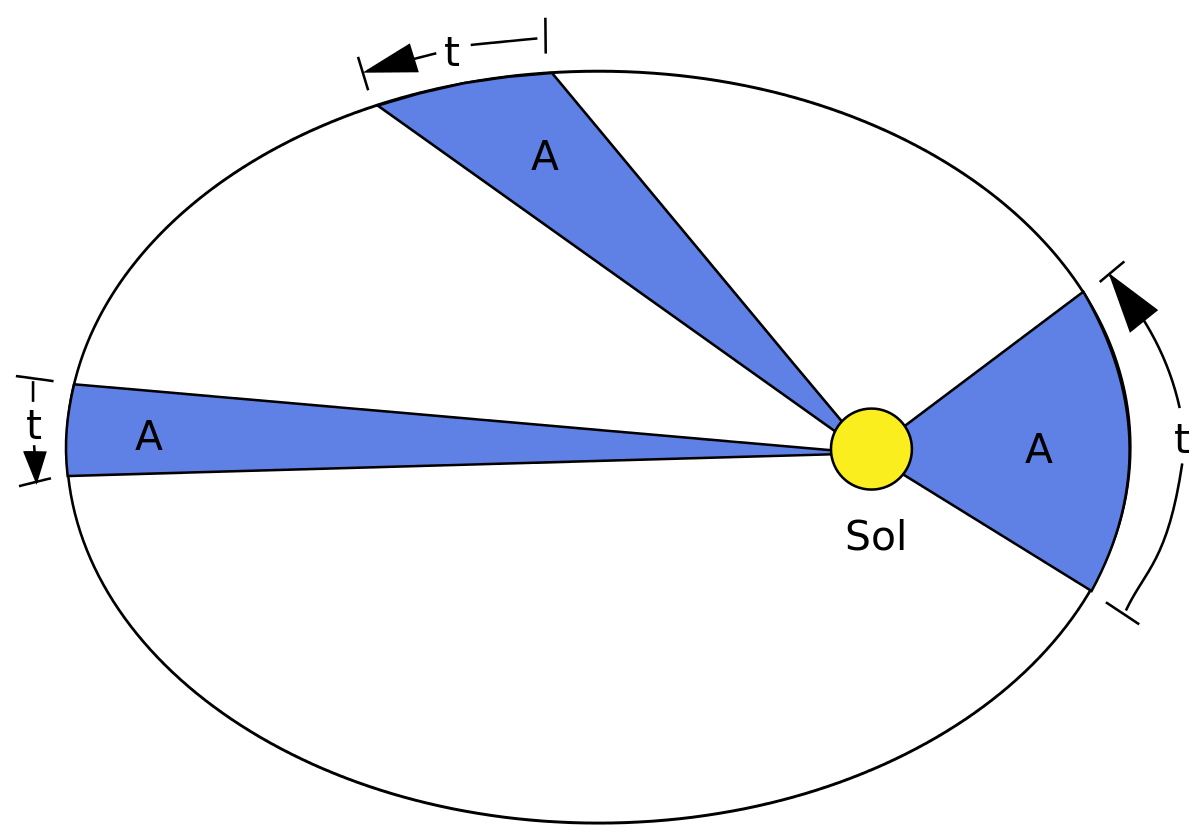
\includegraphics[scale=0.2]{kepler2}
    \item For two planets orbiting around the same sun, $\left( \dfrac{T_1}{T_2} \right)^2 = \left( \dfrac{r_1}{r_2} \right)^3 $
\end{enumerate}

\subsubsection{Period and Energy of Elliptical Orbits}
For elliptical orbits, all equations are the same as for circular orbits but the radius of the circle ($r$) is replaced by $r_a$, the semi-major axis (bigger 'radius' of the ellipse).

\end{document}